\subsection{IDE integration}
\begin{figure}
	\label{fig:idePacmanTop}
	\centering
	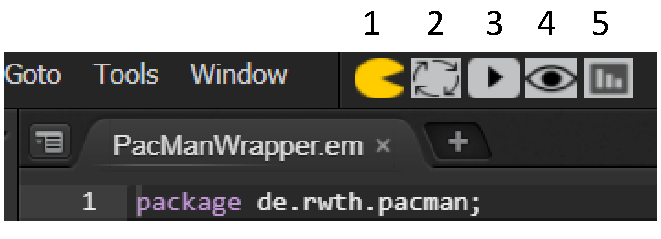
\includegraphics[scale=0.55]{pictures/IDE-PacMan-Top.pdf}
	\caption{Main options for the PacMan project in the ide}
\end{figure}
To integrate a simulator into the EmbeddedMontiArcStudio several steps were necessary. In figure. \ref{fig:idePacmanTop} you can see the top view of the EmbeddedMontiArc's ide. The five added features here are as follows:
\begin{itemize}
	\item[1.] This opens a new tab where you can play a normal game of PacMan
	\item[2.] Generate the WebAssembly of the main component
	\item[3.] This opens a new tab in which the simulation of the component takes place
	\item[4.] Generates the visualization of the main component and shows it in a new tab
	\item[5.] Generates the reporting of all components and shows it in a new tab
\end{itemize}
The features needed to be implemented properly in different places in order to work along the logic of the ide. Each one calls a batch script which again runs the jar for the demanded task for the specific files. In addition, for feature 1 and 2 extra plugins were required which got implemented by group A (expert) and can be reused for SuperMario.
A full list of the files edited can be found in the attachment.

\subsection{Interface}
\begin{figure}
	\label{fig:visPacmanWrapper}
	\centering
	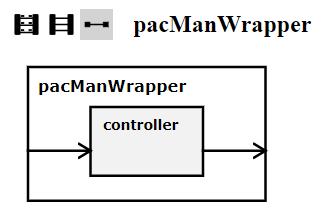
\includegraphics[scale=0.7]{pictures/VisualizationPacManWrapper.png}
	\caption{Visualization of the PacMan wrapper}
\end{figure}
\begin{lstlisting}[label=lst:pacmanWrapper, caption=Interface of the Pacman Wrapper, morekeywords={ports, port, connect, in, out, instance, ->},
frame=single]
ports 
	in Z(0cm: 180cm) ghostX[4],
	in Z(0cm: 210cm) ghostY[4],
	in Z(0 : 1 : 3) ghostDirection[4],
	in B ghostEatable[4],
	in B ghostEaten[4],
	in Z(0cm: 180cm) pacManX,
	in Z(0cm: 210cm) pacManY,
	in B pacManEaten,
	in Z(0:oo) pacManLives,
	in Z(0:oo) pacManScore,
	in Z^{22,19} map,
	out Z(0 : 1 : 3) newPacManDirection;
\end{lstlisting}
The project's main component is PacManWrapper. The main task of the wrapper is to provide a shared interface. Listing \ref{lst:pacmanWrapper} shows the input and output ports. As for the inputs, the ghosts' and the PacMan's position are given, the direction the ghosts are facing, information about the ghosts' vulnerability, as well as the current map. The only output port is the new direction the PacMan should walk. \newline
The wrapper also holds the current controller. This way the controller is easily exchangeable without changing any of the code needed for the ide. All input ports of the wrapper are connected to the corresponding ports of the controller and the output port of the controller is also connected to the output port of the wrapper. \newline
To connect the web assembly of the main component with the PacMan emulator a new JavaScript file was created. Its main functionalities is to extract the needed informations out of the emulator, pass it to the component, execute it and then give the output back to the emulator. In order to be able to extract needed information out of the emulator some modifications were needed. In its original state the emulator did not offer access to the current game object, thus the PACMAN class was extended by these functions. Due to the fact PacMan is a playable game, its input is given as a key-press-event in JavaScript. So the output of the web assembly, which is a number from 0 to 3, is mapped to a corresponding key-press-event which then gets triggered. The emulator is running with 30 frames per second, which also leads to 30 iterations of the game per second. Because the emulator is running asynchronously the component is executed at a double of that rate in order to track every position change.

\subsection{C\&C modeling - PacMan}
\begin{figure}
	\label{fig:visPacmanSimple}
	\centering
	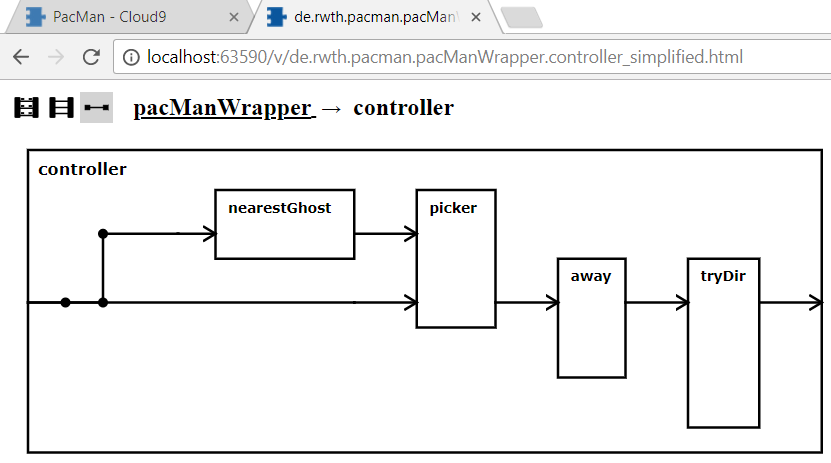
\includegraphics[scale=0.7]{pictures/VisualizationPacManSimple.png}
	\caption{Visualization of the PacMan controller (simple)}
\end{figure}
In fig. \ref{fig:visPacmanSimple} the design of the simple controller is shown. It has four subcomponents:
\begin{itemize}
	\item nearestGhost: Gets the x - and y - position of every ghost and the x - and y - position of the PacMan. It then iterates over all ghosts and calculates the nearest ghost and gives back its index.
	\item picker: Gets all ghost informations as input as well as an index and gives back the ghost information of the ghost at this index.
	\item away: Gets one ghost's informations as well as PacMan's and calculates a new direction for the PacMan facing away from the ghost. The output is one of the four possible directions mapped from the numbers 0 to 3.
	\item tryDir: Gets as input the position of PacMan, the current map as well as a direction the PacMan should try to walk. If there is no wall blocking the way the initial direction is outputted. On the other hand, if there is a wall blocking the way it tries to walk orthogonally left or up. If it fails it will walk right or down respectively.
\end{itemize}
The controller connects the subcomponents in the shown order: It calculates the nearest ghost, passes its index to the picker which then again passes the corresponding ghost to the \textit{away} component. This calculates the direction facing away from said ghost and the \textit{tryDir} component then avoids running into walls. This leads to a controller that runs away from the ghosts with some success but it is only determined by the nearest ghost and has no other goals. Due to the fact that \textit{tryDir} always trys to walk to the left (or top) first, this can lead to some stuttering as soon as the PacMan walked enough to the right that there is again space to the left.
